\documentclass[preprint, prb]{revtex4-1}
\usepackage{amsmath}
\usepackage{amssymb}
\usepackage{graphicx}
\usepackage{enumitem}
\usepackage{bm}
\usepackage[font={footnotesize}]{caption}
\usepackage{todonotes}
\graphicspath{{./}{./images/}}
\definecolor{darkblue}{rgb}{0.1,0.2,0.6} \definecolor{darkred}{rgb}{0.8,0.1,0.2}
\usepackage[colorlinks,citecolor=darkblue,linkcolor=darkred,urlcolor=darkblue]{hyperref}
\usepackage[all]{hypcap}

\renewcommand{\vec}[1]{\boldsymbol{\mathbf{#1}}}

\newcommand{\cf}{\textit{cf.} } 
\newcommand{\ie}{\textit{i.e.} } 
\newcommand{\eg}{\textit{e.g.} }
\newcommand{\vs}{\textit{vs.} } 
\newcommand{\etal}{\textit{et al.} }
\newcommand{\etc}{\textit{etc.} }

\begin{document}

\title{Bipartite Fidelity and Loschmidt echo of bosonic conformal interface}
 
\author{Tianci Zhou}
\email{tzhou13@illinois.edu}
\affiliation{University of Illinois, Department of Physics, 1110 W. Green St. Urbana, IL 61801 USA}

\author{Mao Lin}
\email{maolin2@illinois.edu}
\affiliation{University of Illinois, Department of Physics, 1110 W. Green St. Urbana, IL 61801 USA}

\date{\today}

\begin{abstract}
\end{abstract}

\maketitle

\section{Introduction}
% the last one to be finished.

\section{Bosonic Conformal Interface}
\subsection{General Formulation}
% M, S
% special case
\subsection{Physical Realization: Connecting Bosons of Different Compactification Radii}
% free boson + compact
\subsection{A Free Boson Lattice Model}
% cite Calabrese, introduce the model
% lattice model S matrix

\section{Bipartite Fidelity and Loschmidt Echo}
\subsection{Definition}
% definition
% general discussion

\section{Analytic and Numerical Results}
\subsection{Fidelity}
% analytic: conformal transformation
% numerical comparison 
\subsection{Loschmidt Echo}
% analytic: conformal transformation
% numerical comparison

\section{Discussion}


\begin{acknowledgments}
\todo[inline]{Thomas Faulkner, Xueda Wen, Shinsei Ryu, Romain Vasseur}
    TZ is supported by the National Science Foundation under grant number NSF-DMR-1306011.
    This work made use of the Illinois Campus Cluster, a computing resource that is operated by the
    Illinois Campus Cluster Program (ICCP) in conjunction with the National Center for
    Supercomputing Applications (NCSA) and which is supported by funds from the University of
    Illinois at Urbana-Champaign.
\end{acknowledgments}

\appendix
\section{Corrections to the Free Energy}
% two corrections:
% 1. staircase geometry
% 2. contribution from the boundary: cite Cardy 

\section{Numerical Computation of Bipartite Fidelity and Loschmidt Echo}
% basis transformation, Bogoliubov state, overlap(master theorem)
% Peschel_EE.pdf

\section{A Determinant Identity for the Boundary State Amplitude}
\label{app:pf_of_id}
% copy notes app. C
% flatex input: [pf_of_id.tex]

In this appendix, we provide more details for calculating the amplitude $Z_{ab}$ in Sec.{\bf\color{red}where}. We started to prove the following identity for a real symmetric matrix $M$
\begin{equation}
\label{eq:first_id_app_pf_of_id}
\exp\Big\{- \vec{b}^{\dagger} M \vec{b}  \Big\} \exp \Big\{ \vec{b}^{\dagger} R \bar{\vec{b}}^{\dagger}  \Big\}  = \exp \Big\{ \vec{b}^{\dagger} e^{-M}  R \bar{\vec{b}}^{\dagger}  \Big\} \exp\Big\{- \vec{b}^{\dagger} M \vec{b}  \Big\} 
\end{equation}
where ${\bf b}$ and $\bar{\bf b}$ are vectors of bosonic operators. As emphasized in the {\bf\color{red}main text}, the matrix notation, for example, $\vec{b}^{\dagger} R \bar{\vec{b}}^{\dagger}$ should really mean $\sum_{ij}b^\dagger_iR_{ij}\bar{b}_j^\dagger$ where the dagger does not transpose the vector.  

To prove Eq.~\eqref{eq:first_id_app_pf_of_id}, we first consider the special case where $R=\mathbb{I}$. We diagonalize $M = O^{T} \Lambda O $ and rotate the two sets of boson operators to the diagonal basis
\begin{equation}
  \vec{b}^{\dagger}  M \vec{b} = \vec{d}^{\dagger} \Lambda \vec{d}  \quad \vec{d} = O \vec{b} \quad \vec{\bar{d}}^\dagger = O^T \vec{\bar{b}}^\dagger
\end{equation}
where we understood $\vec{\bar{b}}^\dagger$ is a column vector and independent to $\vec{{b}}^\dagger$. Thus the whole expression can be written as
\begin{equation}
\begin{aligned}
  \exp&\Big\{- \vec{b}^{\dagger} M \vec{b}  \Big\} \exp \Big\{ \vec{b}^{\dagger} \bar{\vec{b}}^\dagger  \Big\}  =  
  \exp\Big\{- \vec{d}^{\dagger} \Lambda \vec{d}  \Big\} \exp \Big\{   \vec{d}^{\dagger} \bar{\vec{d}}^\dagger  \Big\} \\
& = \prod_i  \exp\Big\{- \lambda_i d_i^{\dagger} d_i  \Big\} \exp \Big\{  d_i^{\dagger} \bar{d}_i ^{\dagger}  \Big\}
\end{aligned}
\end{equation}
We recall for $ [X, Y] = sY $, 
\begin{equation}
  e^X e^{Y} = e^{\exp (s ) Y} e^{X}
\end{equation}
which is a solvable case of Baker-Campbell-Hausdorff formula. Upon taking $X = -\lambda_i d_i^{\dagger} d_i$, $Y = d_i^{\dagger} \bar{d}^{\dagger}_i$, we have
\begin{equation}
\label{eq:lambda_commutator}
[- \lambda_i d_i^{\dagger} d_i, d_i ^{\dagger} \bar{d}_i^{\dagger}] =  - \lambda_i  d_i ^{\dagger} \bar{d}_i^{\dagger} 
\end{equation}
and so $s = - \lambda_i$ for each $\lambda_i$. This enable us to commute those exponentials
\begin{equation}
\begin{aligned}
 \exp\Big\{- \vec{b}^{\dagger} M \vec{b}  \Big\} \exp \Big\{  \vec{b}^{\dagger} \bar{\vec{b}}^\dagger  \Big\}   &= \prod_i \exp \Big\{ e^{- \lambda_i }  d^{\dagger}_i \bar{d}^{\dagger}_i  \Big\}  \exp \Big\{-\lambda_i  d^{\dagger}_i d_i  \Big\} \\
 & = \exp \Big\{ \vec{b}^{\dagger} e^{-M}  \bar{\vec{b}}^\dagger  \Big\} \exp\Big\{- \vec{b}^{\dagger} M \vec{b}  \Big\} 
\end{aligned}
\end{equation}
For the general case where $R \neq\mathbb{I}$, we take $\vec{\bar{d}}^* = O^T R \vec{\bar{b}}^*$. This will not change the commutation relation of ${\bf d}$, and the role of $\bar{b}$ is decorative in Eq.~\eqref{eq:lambda_commutator}. Hence the rest of the proof follows the same way. \hfill$\blacksquare$

A direct consequence of Eq.~\eqref{eq:first_id_app_pf_of_id} is the following
\begin{equation}
\label{eq:second_id_in_app_pf_of_id}
Z_{ab} = \langle 0 | \exp\Big\{ \vec{b} R_a^* \vec{\bar{b}}\Big\} \exp\Big\{ - \vec{b}^{\dagger} M  \vec{b} \Big\}   \exp\Big\{  \vec{b}^{\dagger} R_b  \vec{\bar{b}}^{\dagger}\Big\}  |0  \rangle  = \frac{1}{\det( 1- R_a^{\dagger} e^{-M} R_b )} 
\end{equation}
where $|0\rangle$ is the vacuum for ${\bf b}$ and $\bar{\bf b}$. Using the identity we have just proved, 
\begin{equation}
Z_{ab} =   \langle 0 | \exp\Big\{ \vec{b} R_a^* \vec{\bar{b}}\Big\}  \exp \Big\{ \vec{b}^{\dagger} e^{-M}  R_b \bar{\vec{b}}^{\dagger}  \Big\}  |0 \rangle 
\end{equation}
A direct application of the MacMahon master theorem
\begin{equation}
  \langle 0 | \exp \Big\{ \vec{b}_1 X \vec{b}_2 \Big\}  \exp \Big\{ \vec{b}^{\dagger}_1 Y \vec{b}^{\dagger}_2 \Big\}|0  \rangle 
 = \frac{1}{\det(1 - X^T Y )}
\end{equation}
proves Eq.~\eqref{eq:second_id_in_app_pf_of_id}. \hfill$\blacksquare$


%%% Local Variables:
%%% TeX-master: "bCFT_paper"
%%% TeX-PDF-mode: t
%%% End:


\section{$\lambda_1 \rightarrow \lambda_2$ Boundary State Amplitude}
\label{app:lambda_12}
% copy notes app. B

\begin{figure}[h]
\centering
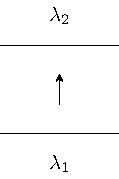
\includegraphics{fig_lambda_1_lambda_2.pdf}
\caption{Partition function between two boundary states of $S_i( \theta_1)$ and that of $S_j( \theta_2 )$}
\label{fig:fig_lambda_1_lambda_2}
\end{figure}

In this appendix, we calculate the amplitude between general boundary states defined in Eq.~\eqref{eq:Zab-bd}
\begin{equation}
\begin{aligned}
Z_{ab} &= \langle 0 | \exp\Big\{  \vec{b} R_b( \theta )    \vec{\bar{b}} \Big\}  \exp\Big\{ -\vec{b}^{\dagger}  (\mathbb{I}_2  \otimes M)  \vec{b} \Big\} \\
&\exp\Big\{  \vec{b}^{\dagger} R_a( \theta )    \vec{\bar{b}}^{\dagger} \Big\} | 0\rangle 
\end{aligned}
\end{equation}
where
\begin{equation}
\begin{aligned}
M &=  \frac{4\pi^2}{\beta} \text{diag}( 1, 2, \cdots ), \quad  \mathbb{I}_2 = \text{diag}( 1, 1) \\
R_i &= S_i( \theta ) \otimes \mathbb{I}
\end{aligned}
\end{equation}
Using the identity Eq.~\eqref{eq:second_id_in_app_pf_of_id} proven in App.~\ref{app:pf_of_id}, we have
\begin{equation}
Z_{ab} = \frac{1}{\det(1 - R_a^{\dagger} ( \mathbb{I}_2 \otimes M ) R_b )}
\end{equation}
From $|\det( R_a R_b^{\dagger})|  = 1$, free energy becomes
\begin{equation}
F = - \ln |Z_{ab}| = \ln |\det ( R_a R_b^{\dagger} - e^{- \mathbb{I}_2 \otimes M} )| .
\end{equation}
There are two cases to be considered, and we only take out the leading order term in $\beta$. 
\begin{itemize}
\item {\it case 1: }$S_1( \theta_1 ) \rightarrow S_2 ( \theta_2 ) $, the free energy is
\begin{equation}
\begin{aligned}
F & = \ln |\det ( R_1( \theta_1 )  R_2^{\dagger}( \theta_2 )  - e^{- \mathbb{I}_2 \otimes M} )| \\
  & = \ln \left| \det
\begin{bmatrix}
-\cos 2 \Delta \theta \mathbb{I} - e^{-M}   & -\sin 2 \Delta \theta \mathbb{I}\\
- \sin 2\Delta \theta \mathbb{I}  &   \cos 2 \Delta \theta \mathbb{I} - e^{-M} \\ 
\end{bmatrix} \right| \\
& = \sum_i \ln [ 1 -  e^{- 2 \lambda_i }  ] \\
& = \frac{\beta}{4\pi^2} \int_0^{\infty} dx \ln [ 1 - e^{-2x} ]  = - \frac{1}{48 }\beta .
\end{aligned}
\end{equation}
\item {\it case 2:} $S_i( \theta_1 ) \rightarrow S_i( \theta_2 )$, where $i = 1 $ or $ 2$, 
\begin{equation}
\begin{aligned}
F & = \ln \det 
\begin{bmatrix}
\cos 2 \Delta \theta \mathbb{I} - e^{-M}   & \sin 2 \Delta \theta \mathbb{I}\\
- \sin 2\Delta \theta \mathbb{I}  &   \cos 2 \Delta \theta \mathbb{I} - e^{-M} \\ 
\end{bmatrix} \\
& = \sum_i \ln [ 1 - 2 \cos 2 \Delta \theta e^{- \lambda_i } + e^{- 2 \lambda_i }  ] \\
& = \frac{\beta}{4\pi^2} \int_0^{\infty} dx \ln [ 1 - 2 \cos 2 \Delta \theta e^{-x} + e^{-2x} ] ,
\end{aligned}
\end{equation}
where $\Delta \theta = \theta_2 - \theta_1$. This integral is an even function of $\Delta \theta$ and the $\Delta \theta > 0$ case reduce to the polylog and Bernoulli polynomial
\begin{equation}
\begin{aligned}
  F &= \frac{\beta}{4\pi^2} \left[ - \text{Li}_2 ( e^{2i |\Delta \theta|} ) - \text{Li}_2 ( e^{- 2i |\Delta \theta|} ) \right] \\
  & = \frac{\beta}{4\pi^2}  \left[ - 2\pi^2 B_2 (|x|) \right] \\
  &= - \frac{\beta}{2} B_2( |x| )  = \frac{\beta}{2} (| x| - x^2 - \frac{1}{6} ),
\end{aligned}
\end{equation}
where $x = \frac{\Delta \theta}{ \pi}$. 
\end{itemize}




%%% Local Variables:
%%% TeX-master: "bCFT_paper"
%%% TeX-PDF-mode: t
%%% End:


\section{Alternative Approach to ${\rm DN} \rightarrow \lambda$ Amplitude}
\label{app:gnd_dn_lambda}
% copy notes app. A
% flatex input: [gnd_dn_lambda.tex]

\begin{figure}[h]
\centering
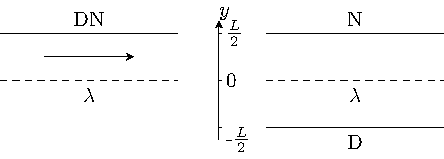
\includegraphics{fig_gnd_dn_lambda.pdf}
\caption{Partition function of Hamiltonian with DN and $\lambda$ boundary conditions. The width of the strip is $\pi$ due to folding. We unfold the cylinder and the new stripe have $N$ and $D$ boundary conditions on the left and right plus a $\lambda$ junction in the middle. }
\label{Fig in gnd_dn_lambda}
\end{figure}

In this appendix, we would like to calculate the amplitude for the setup shown in Fig.~\ref{Fig in gnd_dn_lambda}. In particular, the unfolded configuration has D/N boundary conditions at $x = \pm \frac{L}{2}$ and linking boundary condition at $x = 0$. The general solutions can be written as
\begin{equation}
\label{Normalized f in gnd_dn_lambda}
f(k, x) = 
\left\lbrace
\begin{aligned}
  A_1 e^{i kt} \cos(kx +\frac{1}{2}kL ) &  \quad x < 0  \\
  A_2 e^{ikt}  \sin(kx - \frac{1}{2}kL ) & \quad x > 0   \\
\end{aligned} \right. 
\end{equation}
As demonstrated in the {\bf\color{red}main text}, if we denote $f(k,x<0)\equiv\phi_1$ and $f(k,x>0)\equiv\phi_2$, the boundary condition at the junction reads
\begin{eqnarray}\begin{aligned}
\frac{\partial_x \phi_1}{ \partial_t \phi_1} = \lambda^2 \frac{\partial_x \phi_2}{ \partial_t \phi_2} = \tan^2 \theta\frac{\partial_x \phi_2}{ \partial_t \phi_2} \quad \theta \in [0,\frac{\pi}{2} ]  
\end{aligned}\end{eqnarray}
which implies
\begin{equation}
\label{Momentum in gnd_dn_lambda}
k = \frac{2\pi}{L}( n \pm \frac{\theta}{\pi} )  \quad n\in{\bf Z}
\end{equation}
It is evident that the momentum $k$ is shifted from integer multiple of $2\pi/L$ due to the $\lambda$ boundary condition in the middle. 
\begin{comment}
Thus, the normalized eigenfunctions are
\begin{equation}
f_n(x) = \sqrt{\frac{2}{L}}
\left\lbrace
\begin{aligned}
  \cos(kx +\frac{1}{2}kL ) &  \quad x < 0  \\
  \pm \sin(kx - \frac{1}{2}kL ) & \quad x > 0   \\
\end{aligned} \right. 
\qquad 
k = \frac{2\pi}{L}( n \pm  \frac{\theta}{\pi} )  \quad n \in \mathbb{Z} 
\end{equation}
Expand the field $\phi = \sum_n \phi_n f_n(x) $, the action and Hamiltonian becomes
\begin{equation}
  S = \frac{g}{2} \int dt \, \sum_{n \in \mathbb{Z} }\left(  \dot{\phi}^2_n + k^2 \phi_n^2 \right) \implies\quad   g \dot{\phi}_n  = \pi_n \quad \implies H =  
\frac{1}{2g}\sum_{n \in \mathbb{Z} } \pi_n^2 + ( kg )^2  \phi_n^2 
\end{equation}
\end{comment}

It is clear that the normalized eigenfunctions in Eq.~\eqref{Normalized f in gnd_dn_lambda} serves as orthonormal basis in mode expansion. Following the same procedure in \onlinecite{di_francesco_conformal_1997}, we have the Hamiltonian as
\begin{equation}
\label{H in gnd_dn_lambda}
H = \frac{1}{2} \sum_{n \in \mathbb{Z} } |k|  (a^{\dagger}_n a_n + \frac{1}{2} )
\end{equation}
where the momentum $k$ is defined in Eq.~\eqref{Momentum in gnd_dn_lambda}, and the creation and annihilation operators defined as usual
\begin{equation}
\begin{aligned}
a_n = \frac{1}{\sqrt{2}} ( \sqrt{ |k|g} \phi_n + \frac{i }{\sqrt{|k|g} }\pi_n  ) \\
a^{\dagger}_n = \frac{1}{\sqrt{2}} ( \sqrt{ |k|g} \phi_n - \frac{i }{\sqrt{|k|g} }\pi_n  ) \\
\end{aligned}
\end{equation}

The Casimir energy is the vacuum energy brought by the finite size of the setup. From Eq.~\eqref{H in gnd_dn_lambda} and define $x\equiv\theta/\pi$ in Eq.~\eqref{Momentum in gnd_dn_lambda}, we have
\begin{equation}
\begin{aligned}
E_c &= \frac{1}{4} \sum_{n \in \mathbb{Z}} | k| = \frac{\pi}{2L} ( \sum_{n \in \mathbb{Z}}  | n + x | + \sum_{n \in \mathbb{Z}}  | n - x |  ) \\  
&= \frac{\pi}{L} \Big[\sum_{n \ge 0 } ( n + x )^{-s} + \sum_{n \ge 0 }  ( n - x)^{-s}  +   x^{-s} \Big]\Big|_{s = -1} \\
&= \frac{\pi}{L} \left[ \zeta_{\rm H}( -1, x ) + \zeta_{\rm H}( -1, x ) +  x \right] \\
&= \frac{1}{2} ( - x^2 + x - \frac{1}{6})
\end{aligned}
\end{equation}
where we used the fact that the unfolded geometry has length $L=2\pi$. Thus the free energy reads
\begin{equation}
F = \beta E_c = - \frac{\beta}{2} B_2( x) 
\end{equation}
which agrees with the boundary state calculation in Eq.{\bf\color{red}where}



\bibliographystyle{plain}
\bibliography{bCFT}

\end{document}

%%% Local Variables: 
%%% TeX-PDF-mode: t
%%% End: 
